\documentclass[a4paper,12pt]{article} % тип документа
\usepackage[margin=1in]{geometry} % Поля

%  Русский язык
\usepackage[warn]{mathtext}
\usepackage[T2A]{fontenc}			% кодировка
\usepackage[utf8]{inputenc}			% кодировка исходного текста
\usepackage[english,russian]{babel}	% локализация и переносы
% Математика
\usepackage{amsmath,amsfonts,amssymb,amsthm,mathtools} 
\usepackage{wasysym}
%%%
\usepackage{graphicx}

\usepackage{tabularx}

\usepackage{gensymb} % знак градуса
\usepackage{enumitem} % изменить список enumerate
\usepackage{placeins} % \FloatBarrier

\renewcommand{\thesection}{\Roman{section}} 
\renewcommand{\thesubsection}{\roman{subsection}}
\renewcommand{\thesubsubsection}{\roman{subsection}.\roman{subsubsection}}


\begin{document}

\newcolumntype{Y}{>{\centering\arraybackslash}X} %new tabularx


%титул

\begin{center}
{\LARGE Московский Физико-Технический Институт}
\\
{\large Физтех-школа электроники, фотоники и молекулярной физики }
\\
\vspace{8cm}
{\LARGE Отчёт по лабораторной работе:}
\\
{\Huge Конвективная диффузия в молекулярно- электронных преобразователях} 
\\
\vspace{5cm}
\raggedright 
\hspace{8cm}{\large Выполнил студент группы Б04-005}\\
\hspace{8cm}{\large Карташов Констанин}

\vspace{\fill}
\center
{\large Долгопрудный 2022}

\end{center}

\newpage


\section{Анотация}

\paragraph{Цель работы:} 
Изучение принципа работы молекулярно-электронного преобразователя. Снятие ВАХ и АЧХ.

\paragraph{Оборудование:}
\begin{itemize}
\renewcommand{\labelitemi}{$\triangleright$}
\itemsep0em
\item Молекулярно-электронный преобразователь,
\item АЦП и ЦАП,
\item ПК для снятия показаний.
\end{itemize}


\medskip\hrule\medskip

\section{Теоретическая часть}

\subsection{Молекулярно-электронный преобразователь}

\begin{figure}[h]
\centering
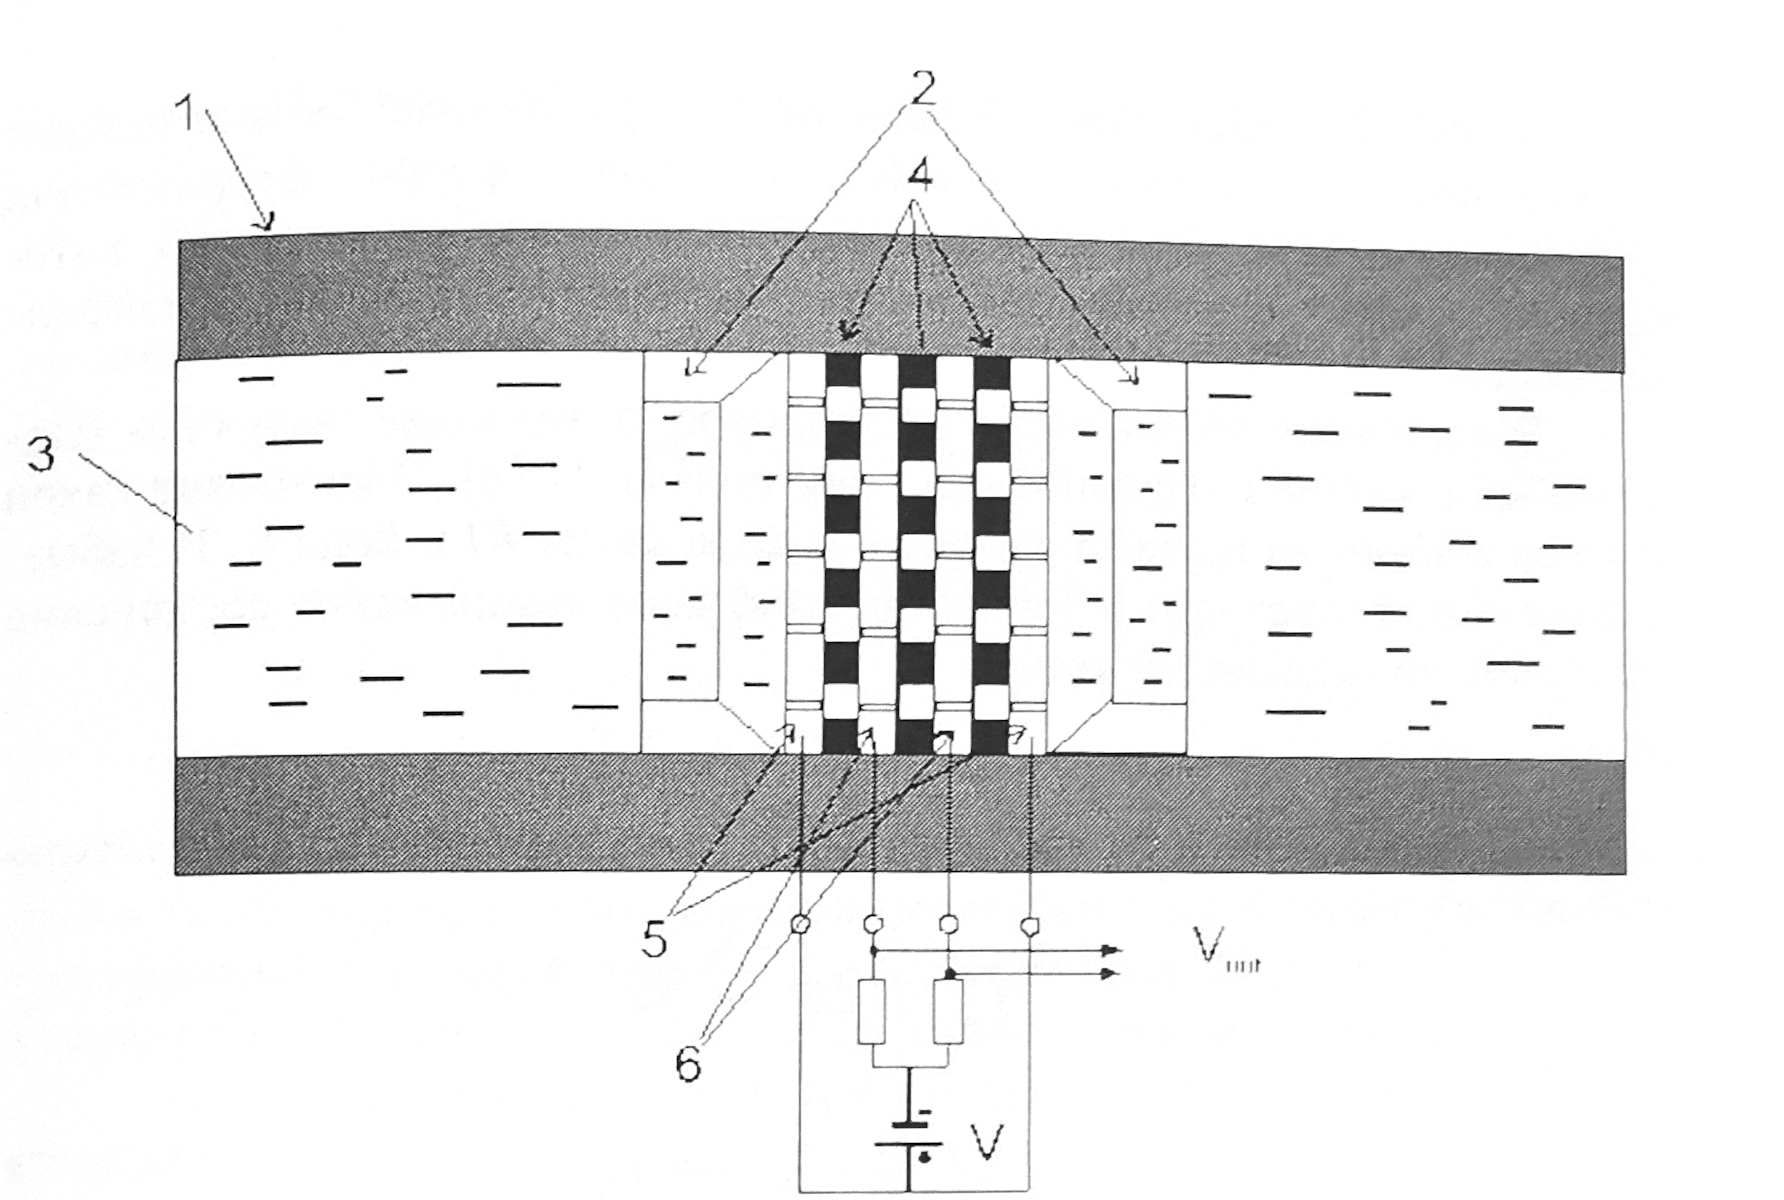
\includegraphics[width=0.7\textwidth]{setup.png}
\caption{Схема молекулярно-электронного преобразователя}
\label{fig:setup}
\end{figure}

\paragraph{} Схема молекулярно-электронного преобразователя (МЭП) представлена на рис. \ref{fig:setup}. МЭП состоит из:
\begin{enumerate}
\itemsep-0.5em
\item Диэлектрической трубки
\item Электродного узла
\item Раствора электролита
\item Пористых перегородок
\item Анодов
\item Катодов
\end{enumerate}

\subsection{Основные физические принципы}

\paragraph{} МЭП заполнен раствором йодита калия (KI). На катоде МЭП происходит восстановление йода:

\[ I_3^- + 2e \; \rightarrow \; 3I^- ,\]

\noindent а на аноде окисление:

\[ 3I^- - 2e \rightarrow I_3^- \].

\paragraph{} Состояние системы описывается уравнениями гидродинамики и диффузии:

\[
\frac{\partial \vec{v}}{\partial t} + (\vec{v} \, \nabla)\vec{v} = - \frac{\nabla p}{\rho} + \gamma \vec{v},
\]
\[
\nabla \cdot \vec{v} = 0,
\]
\[
\frac{\partial C}{\partial t} = D \Delta C + (\vec{v} \cdot \nabla)n.
\]

Уравнение конвективной диффузии:

\[ \frac{\partial C}{\partial t} + \vec{v} \cdot \vec{\nabla} C = D \Delta C.
\]



\medskip\hrule\medskip

\section{Экспериментальная часть}

\subsection{ВАХ молекулярно-электронного преобразователя}

\paragraph{} Будем изменять напряжение на ЦАП, и следить за тем как изменяется показания на АЦП. После стабилизации напряжения на АЦП, зафиксируем значения. Простоим график ВАХ (рис. \ref{fig:vac}).

\begin{figure}[h]
\centering
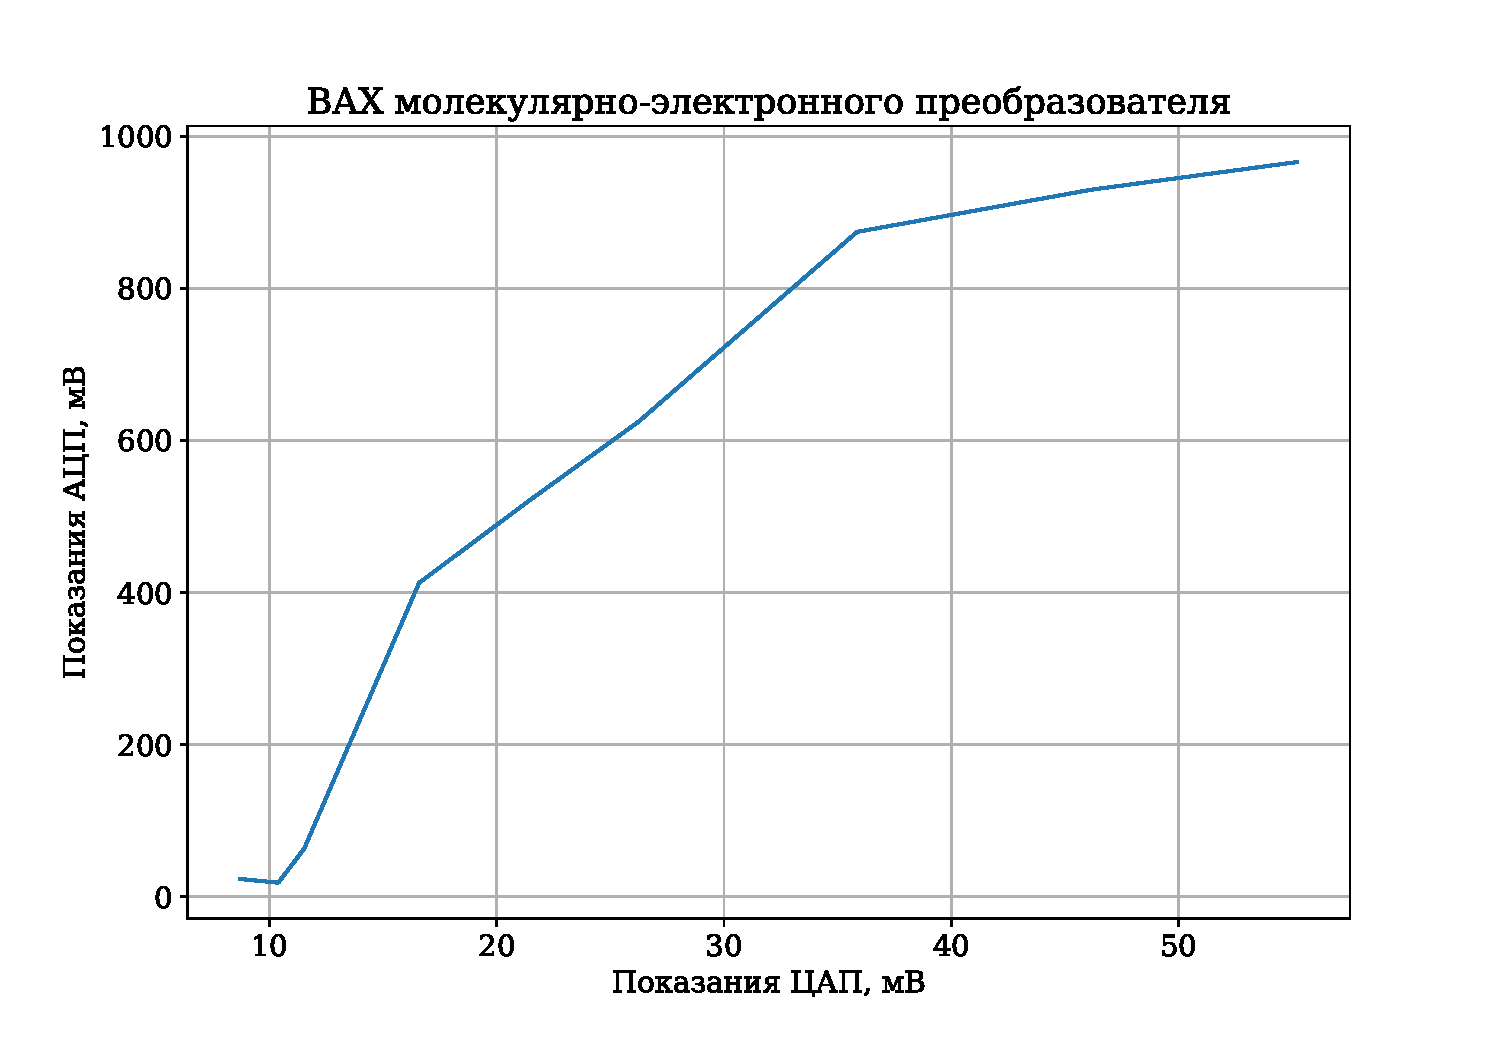
\includegraphics[width=\textwidth]{vac.pdf}
\caption{}
\label{fig:vac}
\end{figure}


\subsection{ЦАП молекулярно-электронного преобразователя}

\paragraph{} Подадим на ЦАП переменное напряжение. Снимем напряжение на АЦП. Построим график зависимости амплитуды колебаний от частоты (рис. \ref{fig:afc}). Также построим логарифмический график (рис. \ref{fig:afc_log}).

\begin{figure}[h]
\centering
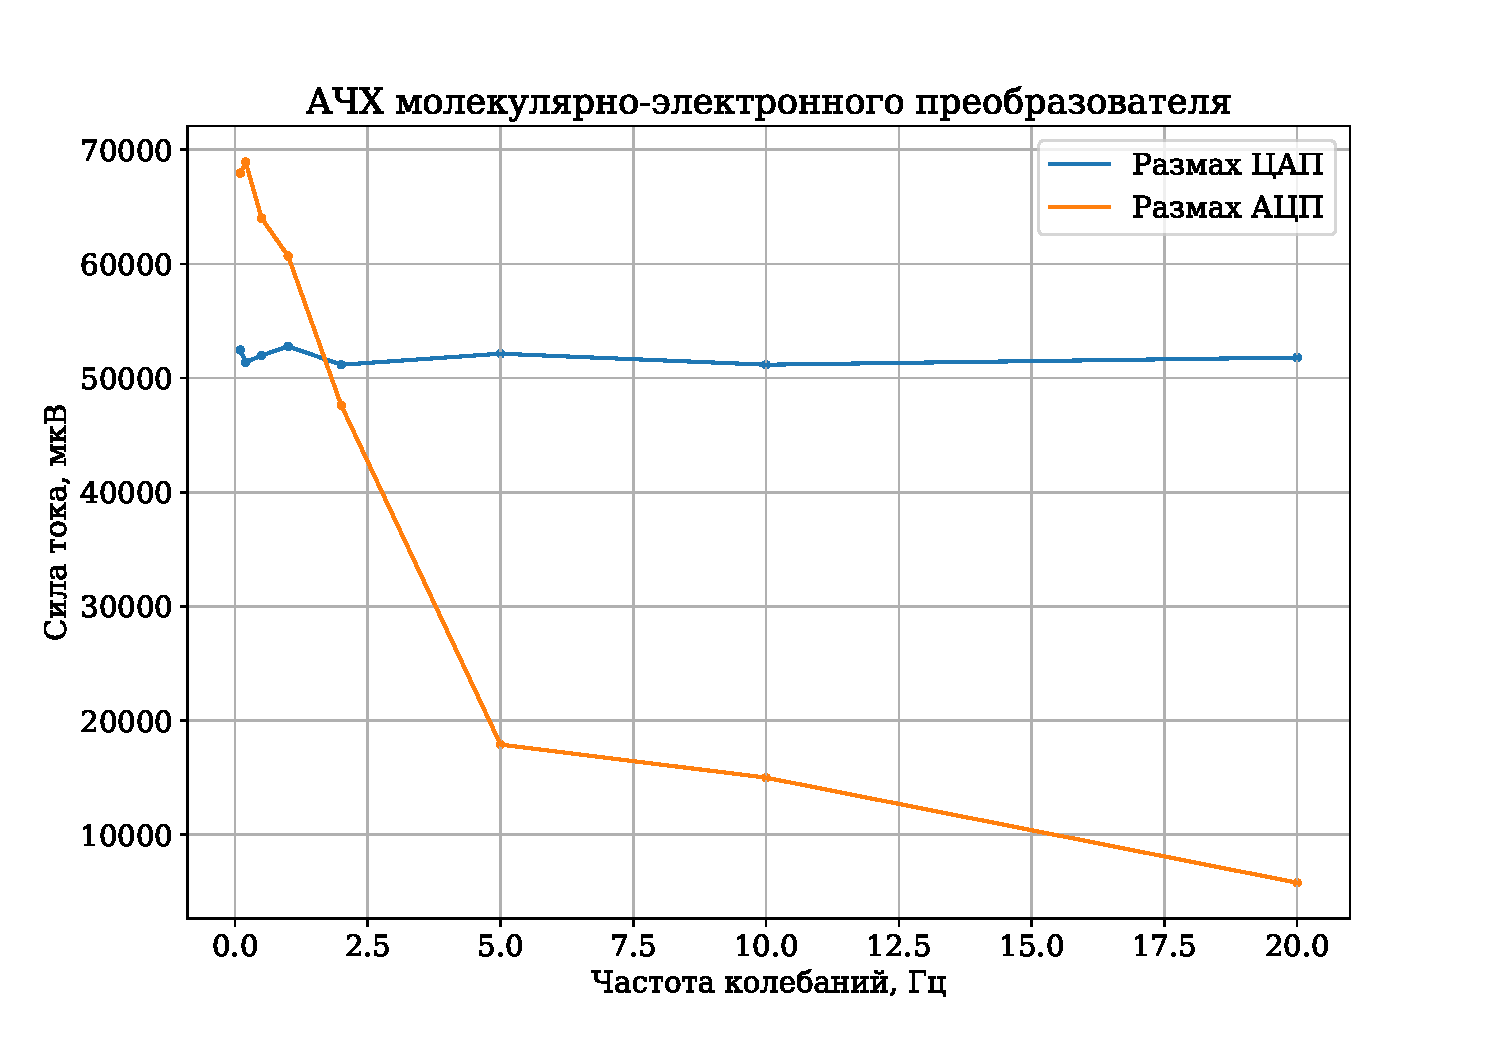
\includegraphics[width=\textwidth]{afc.pdf}
\caption{}
\label{fig:afc}
\end{figure}

\begin{figure}
\centering
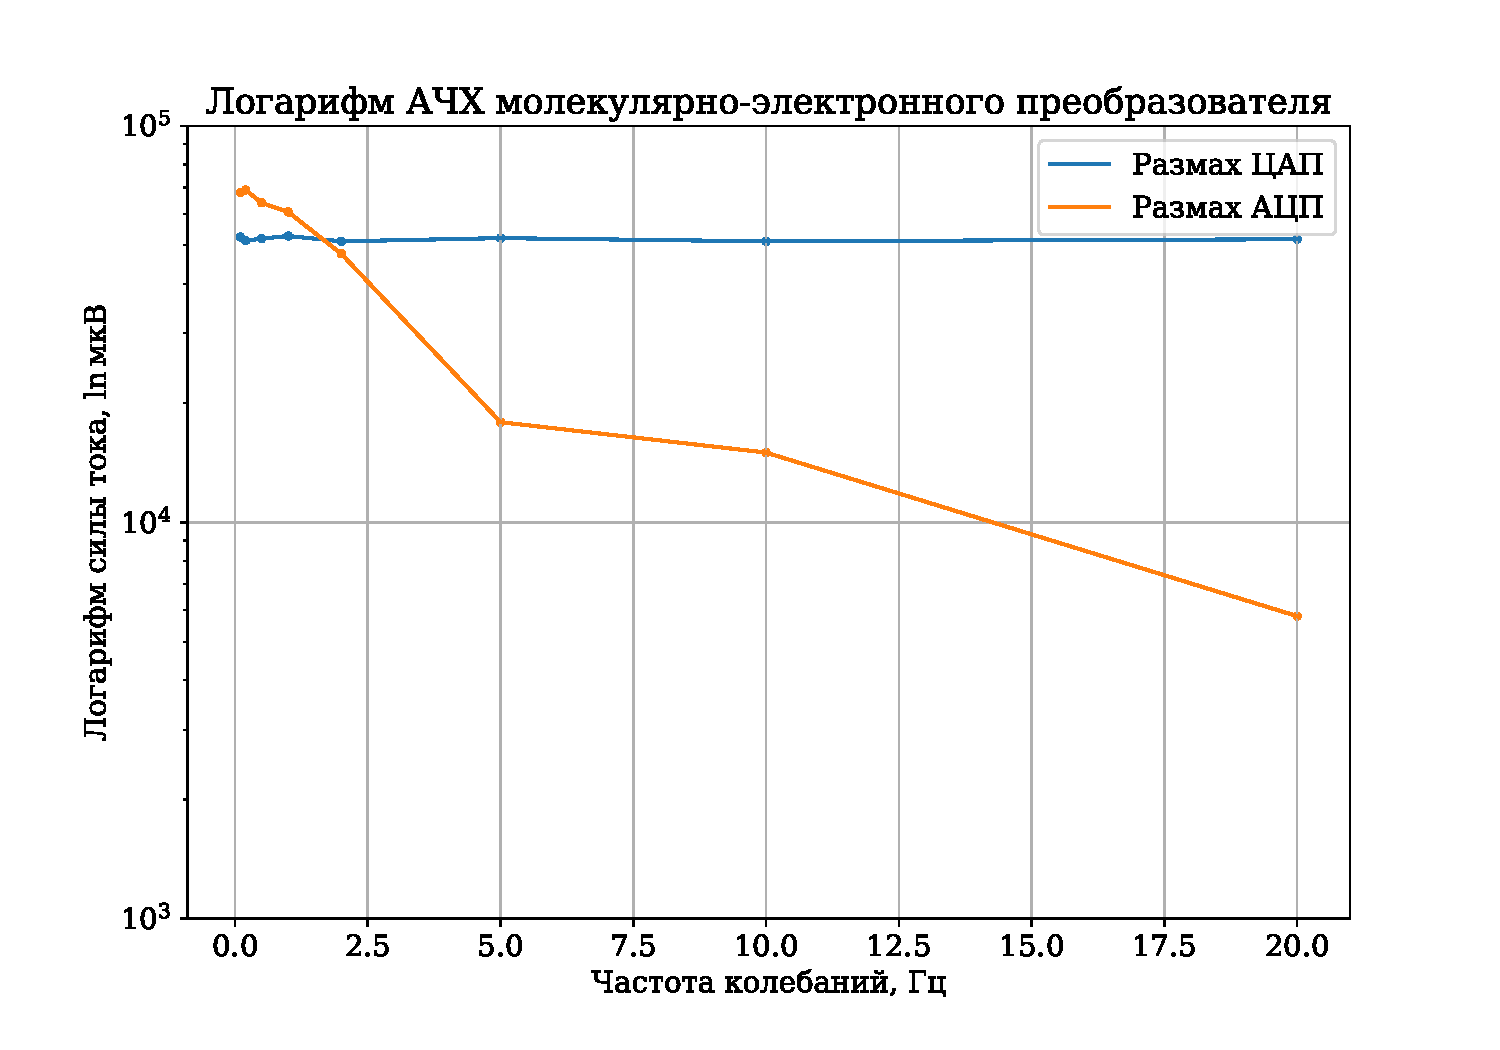
\includegraphics[width=\textwidth]{afc_log.pdf}
\caption{}
\label{fig:afc_log}
\end{figure}


\medskip\hrule\medskip


\end{document}
